\documentclass[11pt]{article}
\usepackage[utf8]{inputenc}
\usepackage{amsmath,amssymb}
\usepackage{geometry}
\usepackage{tikz}
\usepackage{listings}
\usepackage{xcolor}
\usepackage{booktabs}
\usepackage{enumitem}
\usepackage{float}
\usepackage[colorlinks=true, linkcolor=blue!70!black, citecolor=green!50!black, urlcolor=blue!60!black]{hyperref}
\usepackage{cleveref}

\usetikzlibrary{calc, angles, quotes, patterns, arrows.meta, decorations.markings, positioning}

\geometry{letterpaper, margin=1in}

% ── Code listing style ───────────────────────────────────────────────
\definecolor{codebg}{rgb}{0.95, 0.95, 0.95}
\definecolor{codegray}{rgb}{0.4, 0.4, 0.4}
\definecolor{codepurple}{rgb}{0.58, 0.0, 0.82}
\definecolor{codeblue}{rgb}{0.13, 0.13, 1}
\definecolor{codegreen}{rgb}{0.0, 0.5, 0.0}

\lstdefinelanguage{JavaScript}{
  keywords={break, case, catch, continue, debugger, default, delete, do, else,
            false, finally, for, function, if, in, instanceof, new, null, return,
            switch, this, throw, true, try, typeof, var, void, while, with,
            let, const},
  morecomment=[l]{//},
  morecomment=[s]{/*}{*/},
  morestring=[b]',
  morestring=[b]",
  keywordstyle=\color{codeblue}\bfseries,
  identifierstyle=\color{black},
  commentstyle=\color{codegreen}\ttfamily,
  stringstyle=\color{codepurple}\ttfamily,
  sensitive=true
}

\lstset{
  language=JavaScript,
  backgroundcolor=\color{codebg},
  basicstyle=\footnotesize\ttfamily,
  showstringspaces=false,
  numbers=left,
  numberstyle=\tiny\color{codegray},
  numbersep=9pt,
  tabsize=2,
  breaklines=true,
  captionpos=b,
  frame=single,
  rulecolor=\color{codegray!40}
}

% ── Shortcuts ─────────────────────────────────────────────────────────
\newcommand{\code}[1]{\texttt{#1}}
\newcommand{\file}[1]{\texttt{#1}}
\newcommand{\key}[1]{\textsf{\textbf{#1}}}

\title{\textbf{ISSF Rifle Sighting Simulator}\\[4pt]
       \large Mathematical Foundation, Physics Reference, and User Guide}
\author{Documentation for \texttt{simulator.js} / \texttt{index.html}}
\date{April 2026}

% ══════════════════════════════════════════════════════════════════════
\begin{document}
\maketitle
\tableofcontents
\clearpage

% ══════════════════════════════════════════════════════════════════════
\section{Introduction}\label{sec:intro}
% ══════════════════════════════════════════════════════════════════════

The ISSF Rifle Sighting Simulator is a browser-based pedagogical tool
that models the optical and ballistic phenomena encountered in
precision rifle marksmanship.  In ISSF competition, the ``sight
picture'' is not a static image but a dynamic alignment of four
independent planes: the shooter's eye, the rear diopter aperture, the
front globe sight, and the target~\cite{nra,issf}.

The simulator allows students and athletes to isolate, vary, and
observe six fundamental effects that are difficult to separate on the
range:

\begin{enumerate}[nosep]
  \item \textbf{Parallax error}---how head position relative to the
        rear aperture shifts the point of impact
        (\cref{sec:parallax}).
  \item \textbf{Aperture and eye-relief optics}---how diopter size and
        distance affect depth of field and parallax sensitivity
        (\cref{sec:aperture}).
  \item \textbf{Exterior ballistics}---gravity drop over the
        projectile's time of flight (\cref{sec:ballistics}).
  \item \textbf{The canting paradox}---why tilting the rifle
        introduces \emph{both} a lateral shift and a vertical drop
        (\cref{sec:cant}).
  \item \textbf{Mechanical sight adjustment}---how ``clicks'' on the
        front sight translate into impact shifts on the target
        (\cref{sec:clicks}).
  \item \textbf{Wind drift}---lateral and vertical deflection caused
        by atmospheric conditions (\cref{sec:wind}).
\end{enumerate}

\noindent Each phenomenon is developed in its own section with the
competitive-shooting context, a physical explanation, a mathematical
derivation, a reference to the implementing JavaScript code, and
suggested exercises with the simulator.

% ══════════════════════════════════════════════════════════════════════
\section{User Manual}\label{sec:manual}
% ══════════════════════════════════════════════════════════════════════

\subsection{Running the Simulator}
Open \file{index.html} in any modern web browser. The page loads
\file{simulator.js}, which renders the simulation onto an HTML5
\code{<canvas>} element at 1000\,$\times$\,600 pixels. No server or
build step is required.

\subsection{Interface Layout}\label{sec:layout}
The canvas is divided into three regions (\cref{fig:layout}).

\begin{figure}[H]
\centering
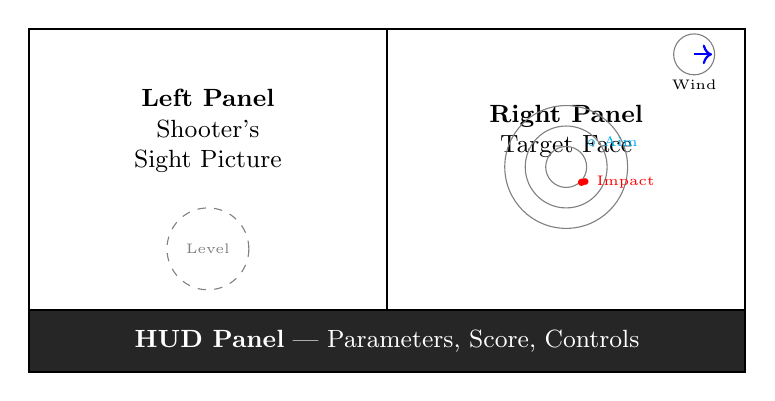
\begin{tikzpicture}[scale=0.65, every node/.style={font=\small}]
  % Left panel
  \draw[thick] (0,0) rectangle (7,5.5);
  \node[align=center] at (3.5,3.5) {\textbf{Left Panel}\\Shooter's\\Sight Picture};
  \draw[dashed,gray] (3.5,1.2) circle (0.8);
  \node[font=\tiny,gray] at (3.5,1.2) {Level};
  % Right panel
  \draw[thick] (7,0) rectangle (14,5.5);
  \node[align=center] at (10.5,3.5) {\textbf{Right Panel}\\Target Face};
  \draw[gray] (10.5,2.8) circle (1.2);
  \draw[gray] (10.5,2.8) circle (0.8);
  \draw[gray] (10.5,2.8) circle (0.4);
  \node[font=\tiny,cyan] at (11.4,3.3) {$\circ$ Aim};
  \filldraw[red] (10.8,2.5) circle (0.06);
  \node[font=\tiny,red] at (11.5,2.5) {$\bullet$ Impact};
  % Wind indicator
  \draw[gray,fill=white] (13,5) circle (0.4);
  \draw[->,blue,thick] (13,5) -- (13.35,5);
  \node[font=\tiny] at (13,4.4) {Wind};
  % HUD
  \draw[thick,fill=black!85] (0,-1.2) rectangle (14,0);
  \node[white,align=center] at (7,-0.6) {\textbf{HUD Panel} --- Parameters, Score, Controls};
\end{tikzpicture}
\caption{Schematic layout of the simulator interface.}
\label{fig:layout}
\end{figure}

\begin{itemize}[nosep]
  \item \textbf{Left panel} (0--500\,px): the shooter's view through
        the rear diopter, showing the front tunnel, iris, target, and
        a spirit-level indicator at the bottom.
  \item \textbf{Right panel} (500--1000\,px): the target face with
        scoring rings. A \textcolor{cyan}{cyan circle} marks the
        parallax-shifted aim point; a \textcolor{red}{red dot} marks
        the predicted impact after all ballistic and mechanical
        corrections.  A wind-direction indicator is displayed in the
        upper-right corner.
  \item \textbf{HUD panel} (bottom 85\,px): numerical readouts of
        all parameters, the decimal score, and a control-key reminder.
\end{itemize}

\subsection{Controls Reference}\label{sec:controls}

\begin{table}[H]
\centering\small
\begin{tabular}{@{}llll@{}}
\toprule
\textbf{Input}       & \textbf{Action}
                      & \textbf{Range}
                      & \textbf{Section} \\
\midrule
Mouse position        & Eye offset (parallax)
                      & canvas area
                      & \cref{sec:parallax} \\
\key{A}\,/\,\key{D}  & Rear aperture $\pm 0.1$\,mm
                      & 0.8--2.2\,mm
                      & \cref{sec:aperture} \\
\key{Q}\,/\,\key{E}  & Front iris $\pm 0.1$\,mm
                      & 2.4--7.0\,mm
                      & \cref{sec:aperture} \\
\key{C}\,/\,\key{V}  & Iris ring thickness $\pm 0.1$\,mm
                      & 0.5--5.0\,mm
                      & \cref{sec:aperture} \\
\key{U}\,/\,\key{J}  & Eye relief $\pm 1$\,mm
                      & 50--215\,mm
                      & \cref{sec:aperture} \\
\key{W}\,/\,\key{S}  & Sight height $\pm 1$\,mm
                      & $\geq 20$\,mm
                      & \cref{sec:ballistics} \\
\key{Z}\,/\,\key{X}  & Rifle cant $\pm 0.57^{\circ}$
                      & unlimited
                      & \cref{sec:cant} \\
Arrow keys            & Mechanical clicks $\pm 1$\,px
                      & unlimited
                      & \cref{sec:clicks} \\
\key{O}\,/\,\key{P}  & Wind speed $\pm 0.5$\,m/s
                      & 0--10\,m/s
                      & \cref{sec:wind} \\
\key{K}\,/\,\key{L}  & Wind direction $\pm 8.6^{\circ}$
                      & full circle
                      & \cref{sec:wind} \\
\key{T}              & Toggle 10\,m / 50\,m target
                      & ---
                      & \cref{sec:ballistics} \\
\key{R}              & Reset all parameters to defaults
                      & ---
                      & --- \\
\key{F}              & Toggle language (English / French)
                      & ---
                      & --- \\
\bottomrule
\end{tabular}
\caption{Complete keyboard and mouse controls.}\label{tab:controls}
\end{table}

\subsection{Quick-Start Walkthrough}\label{sec:quickstart}

\begin{enumerate}[nosep]
  \item Open \file{index.html}. The default view shows a 10\,m air-rifle
        sight picture centered on the target.
  \item Move the mouse across the left panel and observe both the sight picture
        shift and the cyan circle moving on the right panel.  This is
        \emph{parallax} (\cref{sec:parallax}).
  \item Press \key{Z} several times to cant the rifle.  Watch the
        spirit level and the red impact dot on the right panel shift
        right \emph{and} down (\cref{sec:cant}).
  \item Use the arrow keys to bring the red dot back to center---these
        are sight ``clicks'' (\cref{sec:clicks}).
  \item Press \key{T} to switch to the 50\,m target and observe how
        gravity drop and cant error grow dramatically
        (\cref{sec:ballistics}).
  \item Increase wind with \key{P} and rotate its direction with
        \key{K}/\key{L} to see wind drift (\cref{sec:wind}).
\end{enumerate}


% ══════════════════════════════════════════════════════════════════════
\section{Parallax Error}\label{sec:parallax}
% ══════════════════════════════════════════════════════════════════════

\subsection{The Issue for Competitive Shooters}
In ISSF rifle shooting, the shooter views the target through a
small rear diopter aperture.  If the eye is not perfectly centered
behind this aperture, the line of sight through the front sight
projects onto a different point on the target than intended.  This
displacement is called \emph{parallax error}~\cite{nra,mann}.

Even sub-millimeter changes in cheek-weld position can shift the
apparent aim point by a scoring ring or more on the target.  Because
the shooter \emph{perceives} the sights as correctly aligned, the
error is insidious: the sight picture looks acceptable, yet the
point of impact has moved.

\subsection{Why It Matters}
At the 10\,m air-rifle level, a 10.0 versus a 10.5 can determine a
final ranking.  Parallax is the single largest source of shot-to-shot
dispersion for a well-trained athlete whose hold and trigger control
are consistent~\cite{nra}.  Understanding the geometry allows
coaches to diagnose inconsistent groups that are not explained by
natural hold wobble.

\subsection{Physical Explanation and Illustration}

\begin{figure}[H]
\centering
\begin{tikzpicture}[scale=0.78, >=Stealth]
  % Z-axis
  \draw[thick, ->] (-0.5,0) -- (12.5,0) node[right] {$z$};
  % Planes
  \foreach \x/\lab/\zlab in {1/Eye/$z_e$, 3.5/Rear/$z_r$, 11/Target/$z_t$}{
    \draw[dashed, gray] (\x,-2.5) -- (\x,2.5);
    \node[above,font=\small] at (\x,2.5) {\lab};
    \node[below,font=\scriptsize] at (\x,-2.5) {\zlab};
  }
  % On-axis line (reference)
  \draw[gray, thin] (1,0) -- (11,0);
  % Off-axis eye
  \filldraw[blue] (1,1.2) circle (2.5pt) node[left,font=\small] {$E(e_x)$};
  % Line through rear center to target
  \draw[red, thick, ->] (1,1.2) -- (3.5,0);
  \draw[red, thick, dashed] (3.5,0) -- (11,-2.88);
  \filldraw[red] (11,-2.88) circle (2.5pt)
    node[right,font=\small] {$P$ (parallax offset)};
  % Annotations
  \draw[<->,thick,blue] (0.4,0) -- (0.4,1.2) node[midway,left,font=\scriptsize] {$e_x$};
  \draw[<->,thick,red] (11.6,0) -- (11.6,-2.88) node[midway,right,font=\scriptsize] {$p_x$};
  % Similar triangle note
  \node[font=\small,align=center] at (6.5,-3.8)
    {$\displaystyle p_x \;=\; e_x\;\frac{z_r - z_t}{z_r - z_e}$};
\end{tikzpicture}
\caption{Parallax geometry.  An eye offset $e_x$ projects through
the rear-sight center onto the target, producing an error $p_x$ in
the opposite direction, magnified by the distance ratio.}
\label{fig:parallax}
\end{figure}

The line of sight originates at the eye position
$(e_x,\,z_e)$, passes through the center of the rear aperture
$(0,\,z_r)$, and intersects the target plane at~$z_t$.  By the
intercept theorem (similar triangles), the target intersection is:
\begin{equation}\label{eq:parallax}
  p_x = e_x \cdot \frac{z_r - z_t}{z_r - z_e}\,.
\end{equation}
Since $z_t > z_r > z_e$, the fraction is negative, so the parallax
offset on the target is in the \emph{opposite} direction from the
eye displacement and magnified by the ratio of distances.

\subsubsection*{Aperture Damping}
A smaller rear aperture physically blocks off-axis light rays,
constraining the eye to a narrow cone and reducing the range of
parallax offsets that are optically possible~\cite{hecht,smith}.
The simulator models this with a linear damping factor:
\begin{equation}\label{eq:damping}
  f = \max\!\bigl(0.05,\;\tfrac{d_{\text{rear}}}{4.5}\bigr),
  \qquad p_x \leftarrow p_x \cdot f\,,
\end{equation}
where $d_{\text{rear}}$ is the rear aperture diameter in mm.  At the
minimum aperture of 0.8\,mm, $f \approx 0.18$, reducing parallax
sensitivity by roughly 80\,\%.

\subsection{Implementation}\label{sec:parallax-impl}
In \file{simulator.js}, the \code{compute()} function (lines~74--79):
\begin{lstlisting}
const scale = (targetZ - eyeZ) / (rearZ - eyeZ);
let px = eyeXoff + (0 - eyeXoff) * scale;
let py = eyeYoff + (0 - eyeYoff) * scale;

const f = Math.max(0.05, rearAperture_mm / 4.5);
px *= f;  py *= f;
\end{lstlisting}
Here \code{scale} is the ratio $\frac{z_t - z_e}{z_r - z_e}$, and
the expression \code{eyeXoff + (0 - eyeXoff) * scale} evaluates to
$e_x(1 - \text{scale}) = e_x \cdot \frac{z_r - z_t}{z_r - z_e}$,
which is \cref{eq:parallax}.  The aperture damping factor~$f$
(\cref{eq:damping}) is applied to both axes.

\subsection{Simulator Exercises}
\begin{enumerate}[nosep]
  \item With the default 1.6\,mm rear aperture, sweep the mouse across
        the canvas and note the cyan dot displacement on the right
        panel.
  \item Reduce the aperture to 0.8\,mm (\key{A}) and repeat.  The
        cyan dot should move far less---this is the pinhole effect
        (\cref{eq:damping}).
  \item Increase the aperture to 2.2\,mm (\key{D}).  Parallax
        sensitivity rises and the target image becomes blurred
        (see \cref{sec:aperture}).
\end{enumerate}


% ══════════════════════════════════════════════════════════════════════
\section{Aperture Size and Eye Relief}\label{sec:aperture}
% ══════════════════════════════════════════════════════════════════════

\subsection{The Issue for Competitive Shooters}
The rear diopter and front iris form the optical frame of the sight
picture.  Their diameters and the distance from the eye to the rear
sight (\emph{eye relief}) determine three competing properties:
\begin{enumerate}[nosep]
  \item \textbf{Depth of field:} smaller apertures yield sharper images of
        both the front sight and the target, analogous to a pinhole
        camera~\cite{hecht}.
  \item \textbf{Light transmission:} too small an aperture reduces
        brightness and may cause diffraction artifacts, leading to eye
        fatigue.
  \item \textbf{Parallax sensitivity:} as derived in
        \cref{sec:parallax}, smaller apertures reduce the magnitude
        of parallax error.
\end{enumerate}

\subsection{Why It Matters}
Choosing the correct aperture is a balance: too wide and the front
sight ring blurs, degrading centering precision; too narrow and the
image darkens, especially in indoor ranges with poor lighting.  Eye
relief must also be consistent---changes in head position alter the
apparent size of the rear aperture in the sight picture, which
disrupts the concentricity judgment~\cite{nra}.

\subsection{Physical Explanation and Illustration}

\begin{figure}[H]
\centering
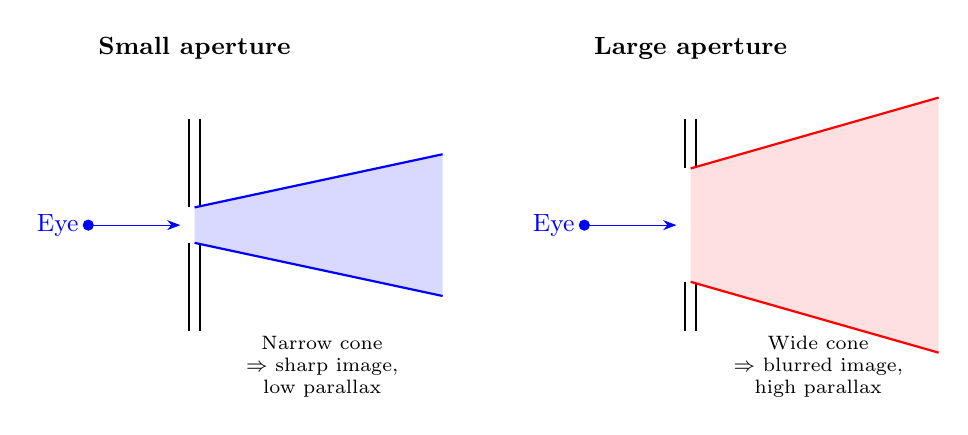
\begin{tikzpicture}[scale=0.9, >=Stealth]
  % --- Small aperture ---
  \node[font=\small\bfseries] at (0,2.5) {Small aperture};
  \draw[thick] (-0.08,1.5) -- (-0.08,0.25);
  \draw[thick] (0.08,1.5) -- (0.08,0.25);
  \draw[thick] (-0.08,-0.25) -- (-0.08,-1.5);
  \draw[thick] (0.08,-0.25) -- (0.08,-1.5);
  % Light cone
  \fill[blue!15] (0,0.25) -- (3.5,1.0) -- (3.5,-1.0) -- (0,-0.25) -- cycle;
  \draw[blue,thick] (0,0.25) -- (3.5,1.0);
  \draw[blue,thick] (0,-0.25) -- (3.5,-1.0);
  % Eye
  \filldraw[blue] (-1.5,0) circle (2pt) node[left,font=\small] {Eye};
  \draw[blue,->] (-1.5,0) -- (-0.2,0);
  \node[font=\scriptsize,align=center] at (1.8,-2) {Narrow cone\\$\Rightarrow$ sharp image,\\low parallax};

  % --- Large aperture ---
  \begin{scope}[xshift=7cm]
    \node[font=\small\bfseries] at (0,2.5) {Large aperture};
    \draw[thick] (-0.08,1.5) -- (-0.08,0.8);
    \draw[thick] (0.08,1.5) -- (0.08,0.8);
    \draw[thick] (-0.08,-0.8) -- (-0.08,-1.5);
    \draw[thick] (0.08,-0.8) -- (0.08,-1.5);
    % Light cone
    \fill[red!12] (0,0.8) -- (3.5,1.8) -- (3.5,-1.8) -- (0,-0.8) -- cycle;
    \draw[red,thick] (0,0.8) -- (3.5,1.8);
    \draw[red,thick] (0,-0.8) -- (3.5,-1.8);
    \filldraw[blue] (-1.5,0) circle (2pt) node[left,font=\small] {Eye};
    \draw[blue,->] (-1.5,0) -- (-0.2,0);
    \node[font=\scriptsize,align=center] at (1.8,-2) {Wide cone\\$\Rightarrow$ blurred image,\\high parallax};
  \end{scope}
\end{tikzpicture}
\caption{Pinhole analogy.  A smaller rear aperture restricts the cone
of accepted light rays, increasing depth of field and reducing
parallax sensitivity.}
\label{fig:aperture}
\end{figure}

\subsubsection*{Apparent Aperture Size and Eye Relief}
The visual angle subtended by the rear diopter from the eye depends
inversely on the relief distance $R = z_r - z_e$:
\begin{equation}\label{eq:apparent-size}
  r_{\text{apparent}} \;\propto\; \frac{d_{\text{rear}}}{R}\,.
\end{equation}
Larger relief makes the aperture appear smaller, narrowing the
visible field, while smaller relief opens the view.  The simulator
implements this in the rendering code as:
\begin{equation}\label{eq:rearR}
  r_{\text{px}} = (d_{\text{rear}} \times 10) \times \frac{250}{R}\,.
\end{equation}

\subsubsection*{Target Blur}
When the rear aperture is large, the depth of field shrinks and the
target image appears blurred.  The simulator applies a Gaussian blur
proportional to the aperture size:
\begin{equation}\label{eq:blur}
  \sigma_{\text{blur}} = \max\!\bigl(0,\;(d_{\text{rear}} - 0.9) \times 4\bigr)\;\text{px}.
\end{equation}

\subsection{Implementation}
In \file{simulator.js}, the rendering function \code{drawLeft()}
(lines~171--173 and~120--121):
\begin{lstlisting}
const relief = Math.max(5, rearZ - eyeZ);
const rearR = (rearAperture_mm * 10) * (250 / relief);
const targetBlur = Math.max(0, (rearAperture_mm - 0.9) * 4);
\end{lstlisting}

The front iris and ring thickness are rendered as concentric arcs
whose radii are proportional to \code{frontIris\_mm} and
\code{frontThickness\_mm}, providing a visual representation of the
three-ring sight picture (rear diopter, front tunnel, front iris).

\subsection{Simulator Exercises}
\begin{enumerate}[nosep]
  \item Start with the default aperture (1.6\,mm).  Press \key{D} to
        widen the rear aperture to 2.2\,mm: note the target blur
        increase and the parallax sensitivity rise.
  \item Press \key{A} to narrow to 0.8\,mm: the image sharpens and
        darkens, and parallax sensitivity drops.
  \item Use \key{U}/\key{J} to change eye relief.  Watch how the
        visible diameter of the sight picture changes
        (\cref{eq:apparent-size}).  A relief that is too short causes
        the rear aperture to fill the view; too long and the front
        tunnel cannot be framed concentrically.
  \item Adjust front iris (\key{Q}/\key{E}) and thickness
        (\key{C}/\key{V}) to explore how the inner ring frames the
        target bull.
\end{enumerate}


% ══════════════════════════════════════════════════════════════════════
\section{Exterior Ballistics: Gravity and Trajectory}\label{sec:ballistics}
% ══════════════════════════════════════════════════════════════════════

\subsection{The Issue for Competitive Shooters}
The line of sight is perfectly straight, but a projectile follows a
parabolic arc under gravity~\cite{mccoy,rinker}.  To make the
bullet hit the point of aim at a given distance, the barrel must be
angled slightly upward relative to the sight line.  The angular
offset depends on the \emph{sight height} (the vertical distance
from bore center to the optical axis of the sights) and the
\emph{gravity drop} at the target distance.

\subsection{Why It Matters}
The total vertical compensation $C = H + h_g$ is the foundation on
which canting error is built (\cref{sec:cant}).  At 50\,m, gravity
drop is an order of magnitude larger than at 10\,m, explaining why
canting and wind errors become far more severe in smallbore
competition.  Understanding the relationship between sight height,
muzzle velocity, and gravity drop helps athletes interpret their
equipment choices~\cite{litz,pejsa}.

\subsection{Physical Explanation and Illustration}

\begin{figure}[H]
\centering
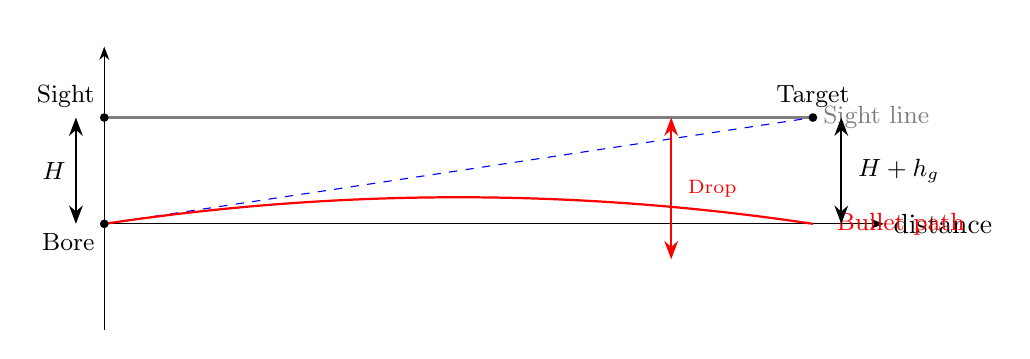
\begin{tikzpicture}[scale=0.9, >=Stealth]
  % Axes
  \draw[->] (0,0) -- (11,0) node[right] {distance};
  \draw[->] (0,-1.5) -- (0,2.5) node[above] {};
  % Sight line
  \draw[gray, thick] (0,1.5) -- (10,1.5) node[right,font=\small] {Sight line};
  % Bore line (angled up)
  \draw[dashed, blue] (0,0) -- (10,1.5);
  \node[blue,font=\small,right] at (10.0,1.1) {};
  % Bullet path (parabola, starts at bore, curves down)
  \draw[red, thick, domain=0:10, samples=50]
    plot (\x, {0 + 0.15*\x + 0*\x - 0.015*\x*\x});
  \node[red,font=\small,right] at (10.2,0) {Bullet path};
  % Sight height
  \draw[<->,thick] (-0.4,0) -- (-0.4,1.5)
    node[midway,left,font=\small] {$H$};
  % Gravity drop at target
  \draw[<->,thick] (10.4,0) -- (10.4,1.5);
  \node[font=\small,right] at (10.5,0.75) {$H + h_g$};
  % Labels
  \filldraw (0,0) circle (1.5pt) node[below left,font=\small] {Bore};
  \filldraw (0,1.5) circle (1.5pt) node[above left,font=\small] {Sight};
  \filldraw (10,1.5) circle (1.5pt) node[above,font=\small] {Target};
  % Drop annotation
  \draw[<->,thick,red] (8,-0.5) -- (8,1.5);
  \node[red,font=\scriptsize,right] at (8.1,0.5) {Drop};
\end{tikzpicture}
\caption{Sight height and gravity drop.  The bore is angled upward by
the combined compensation $C = H + h_g$ so that the parabolic bullet
path intersects the line of sight at the target distance.}
\label{fig:trajectory}
\end{figure}

\subsection{Mathematical Model}
For a projectile with muzzle velocity $v$ fired at a target at
distance $d$, the time of flight is:
\begin{equation}\label{eq:tof}
  t = \frac{d}{v}\,.
\end{equation}
The vertical drop due to gravity during this time is~\cite{mccoy}:
\begin{equation}\label{eq:drop}
  h_g = \frac{1}{2}\,g\,t^2 = \frac{g\,d^2}{2\,v^2}\,.
\end{equation}
The total vertical compensation required at the target is:
\begin{equation}\label{eq:totalcomp}
  C = H + h_g\,,
\end{equation}
where $H$ is the sight height.  Typical values used in the simulator:

\begin{table}[H]
\centering\small
\begin{tabular}{@{}lcccc@{}}
\toprule
\textbf{Discipline} & $d$ (m) & $v$ (m/s) & $t$ (ms) & $h_g$ (mm) \\
\midrule
10\,m Air Rifle  & 10 & 175 & 57.1  & 16.0  \\
50\,m Smallbore  & 50 & 330 & 151.5 & 112.6 \\
\bottomrule
\end{tabular}
\caption{Time of flight and gravity drop for the two target modes.}
\label{tab:drop}
\end{table}

\subsection{Implementation}
In \file{simulator.js}, lines~85--88 of \code{compute()}:
\begin{lstlisting}
const dist_m = targetType === "10m" ? 10 : 50;
const velocity_ms = targetType === "10m" ? 175.0 : 330.0;
const time_s = dist_m / velocity_ms;
const gravityDrop_mm = 0.5 * GRAVITY * (time_s * time_s) * 1000;
\end{lstlisting}
The factor of 1000 converts from metres to millimetres.  The total
compensation $C$ is formed on line~91:
\begin{lstlisting}
const totalComp_mm = sightHeight_mm + gravityDrop_mm;
\end{lstlisting}

\subsection{Simulator Exercises}
\begin{enumerate}[nosep]
  \item In 10\,m mode, note the gravity drop displayed in the HUD
        ($\approx$16\,mm).  Press \key{T} to switch to 50\,m and
        observe the drop increase to $\approx$113\,mm.
  \item Use \key{W}/\key{S} to raise or lower the sight height.
        Observe in \cref{sec:cant} how this changes the sensitivity
        to canting error.
\end{enumerate}


% ══════════════════════════════════════════════════════════════════════
\section{Rifle Cant}\label{sec:cant}
% ══════════════════════════════════════════════════════════════════════

\subsection{The Issue for Competitive Shooters}
\emph{Canting} is the rotation of the rifle about the bore axis---a
tilt to the left or right as viewed from behind.  Because the barrel
must be angled \emph{upward} to compensate for gravity
(\cref{sec:ballistics}), any tilt rotates this vertical compensation
vector out of the vertical plane.  The result is a point-of-impact
error that has \emph{both} a lateral and a vertical component---the
``canting paradox''~\cite{rinker,mann}.

\subsection{Why It Matters}
Even small cant angles produce measurable errors, especially at
longer distances where the total compensation $C = H + h_g$ is
large.  At 50\,m, a 2$^\circ$ cant shifts the impact laterally by
$\approx$\,6\,mm---more than a full scoring ring.  Because the rifle
appears ``almost level'' to the shooter, canting errors are easy to
introduce and difficult to detect without a spirit level.  The impact
\textbf{always drops} and shifts \textbf{toward the direction of
the cant}~\cite{nra,rinker}.

\subsection{Physical Explanation and Illustration}

\begin{figure}[H]
\centering
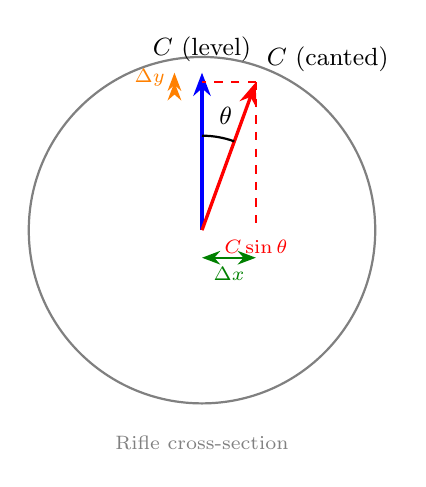
\begin{tikzpicture}[scale=1.0, >=Stealth]
  % Rifle circle
  \draw[thick, gray] (0,0) circle (2.2);
  \node[gray,font=\scriptsize] at (0,-2.7) {Rifle cross-section};

  % Uncanted compensation vector
  \draw[very thick, blue, ->] (0,0) -- (0,2.0)
    node[above,font=\small,black] {$C$ (level)};

  % Canted compensation vector (20 degrees for visibility)
  \draw[very thick, red, ->] (0,0) -- ({2.0*sin(20)},{2.0*cos(20)})
    node[above right,font=\small,black] {$C$ (canted)};

  % Decomposition
  \draw[dashed, red, thick] ({2.0*sin(20)},{2.0*cos(20)}) -- ({2.0*sin(20)},0)
    node[below,font=\scriptsize] {$C\sin\theta$};
  \draw[dashed, red, thick] ({2.0*sin(20)},{2.0*cos(20)}) -- (0,{2.0*cos(20)});

  % Vertical loss
  \draw[<->,thick,orange] (-0.35,{2.0*cos(20)}) -- (-0.35,2.0);
  \node[orange,font=\scriptsize,left] at (-0.35,{(2.0+2.0*cos(20))/2}) {$\Delta y$};

  % Angle arc
  \draw[thick] (0,1.2) arc (90:{90-20}:1.2);
  \node[font=\small] at (0.3,1.45) {$\theta$};

  % Horizontal error
  \draw[<->,thick,green!50!black] (0,-0.35) -- ({2.0*sin(20)},-0.35);
  \node[green!50!black,font=\scriptsize,below] at ({1.0*sin(20)},-0.35) {$\Delta x$};
\end{tikzpicture}
\caption{The canting paradox.  When the rifle is tilted by $\theta$,
the compensation vector~$C$ rotates, producing a lateral error
$\Delta x = C\sin\theta$ and a vertical loss
$\Delta y = C(1-\cos\theta)$.}
\label{fig:cant}
\end{figure}

\subsection{Mathematical Model}
When the rifle is level, the bore-to-sight compensation vector is
purely vertical: $(0,\,C)$.  When the rifle is canted by angle
$\theta$, this vector rotates to $(C\sin\theta,\;C\cos\theta)$.
The errors on the target, relative to the uncanted aim point,
are~\cite{rinker,mann}:
\begin{align}
  \Delta x &= C\,\sin\theta \,,          \label{eq:cant-x}\\
  \Delta y &= C\,(1 - \cos\theta) \,,    \label{eq:cant-y}
\end{align}
where $\Delta x$ is the lateral shift (positive in the direction of
the cant) and $\Delta y$ is the vertical drop (always
positive---impact always falls).

For small angles ($\theta \ll 1$), the approximations
$\sin\theta \approx \theta$ and $1 - \cos\theta \approx
\theta^2/2$ reveal that the lateral error is first-order in $\theta$
while the vertical drop is second-order.  This explains the
well-known observation that cant primarily causes horizontal
dispersion at small angles.

\subsubsection*{Numerical Example}
At 50\,m ($C = 60 + 112.6 = 172.6$\,mm), a cant of
$\theta = 2^\circ$ ($0.0349$\,rad):
\begin{align*}
  \Delta x &= 172.6 \times \sin(0.0349) = 6.0\;\text{mm}\,,\\
  \Delta y &= 172.6 \times (1 - \cos(0.0349)) = 0.1\;\text{mm}\,.
\end{align*}
The horizontal shift is 60$\times$ larger than the vertical drop,
consistent with competitive experience.

\subsection{Implementation}\label{sec:cant-impl}
In \file{simulator.js}, lines~91--93 of \code{compute()}.  The cant
errors are computed in \textbf{canvas coordinates} where $+y$~points
downward, so a positive \code{shiftY\_mm} moves the impact
downward on screen (i.e., the impact drops, as expected physically):
\begin{lstlisting}
const totalComp_mm = sightHeight_mm + gravityDrop_mm;
const shiftX_mm = totalComp_mm * Math.sin(cant);
const shiftY_mm = totalComp_mm * (1 - Math.cos(cant));
\end{lstlisting}

\noindent\textbf{Note on coordinate convention.}
In a standard mathematical frame ($+y$ up), the vertical error is
$C(\cos\theta - 1) \leq 0$ (negative means downward).  In the HTML5
Canvas frame ($+y$ down), the same physical drop corresponds to a
\emph{positive} pixel offset.
\Cref{eq:cant-y} is expressed in the canvas convention used by the
implementation: $\Delta y = C(1-\cos\theta) \geq 0$.

\subsection{Simulator Exercises}
\begin{enumerate}[nosep]
  \item In 10\,m mode, press \key{X} several times to introduce a
        clockwise cant.  Observe the red dot shift right and slightly
        down on the right panel, and the spirit-level indicator move
        in the left panel.
  \item Press \key{T} to switch to 50\,m and repeat.  The same cant
        angle produces a much larger lateral shift because $C$ is
        larger.
  \item Increase sight height with \key{W} and note how this
        amplifies the cant error (larger $C$ in
        \cref{eq:cant-x,eq:cant-y}).
  \item Use the arrow keys to zero-out the cant error with clicks
        (\cref{sec:clicks}), then remove the cant with \key{Z}.  The
        impact now moves to the opposite side---demonstrating why
        zeroing under a cant and then removing it doubles the error.
\end{enumerate}


% ══════════════════════════════════════════════════════════════════════
\section{Mechanical Sight Adjustment (Clicks)}\label{sec:clicks}
% ══════════════════════════════════════════════════════════════════════

\subsection{The Issue for Competitive Shooters}
After establishing a natural point of aim, the shooter adjusts the
front sight to bring the group center onto the target center.
These adjustments---commonly called ``clicks'' because many
mechanisms produce an audible click per increment---physically
displace the front-sight element relative to the barrel, changing
the angle between the bore and the line of sight~\cite{nra}.

\subsection{Why It Matters}
Correct use of sight adjustments is essential for zeroing and for
responding to changing conditions (wind, light, temperature).
Understanding the \emph{lever-arm geometry} helps the shooter
predict how many clicks are needed for a given correction and why
front-sight adjustments move the group in the \emph{same} direction
as the adjustment.

\subsection{Physical Explanation and Illustration}

\begin{figure}[H]
\centering
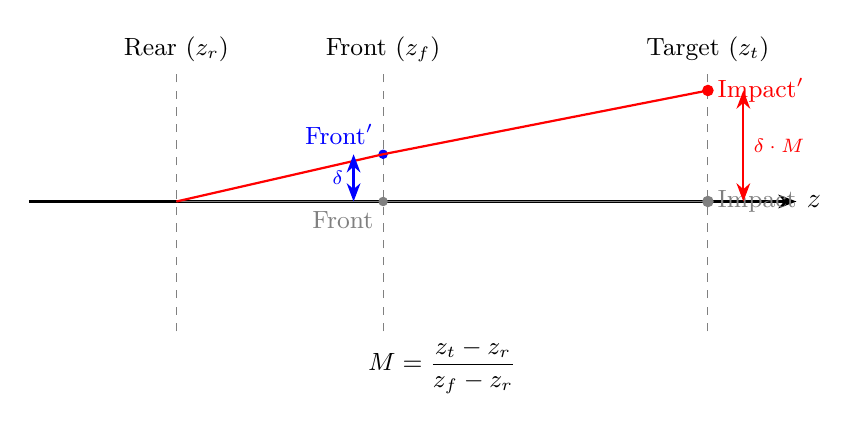
\begin{tikzpicture}[scale=0.75, >=Stealth]
  \draw[thick, ->] (-0.5,0) -- (12.5,0) node[right] {$z$};
  % Planes
  \draw[dashed,gray] (2,-2.2) -- (2,2.2);
  \node[above,font=\small] at (2,2.2) {Rear ($z_r$)};
  \draw[dashed,gray] (5.5,-2.2) -- (5.5,2.2);
  \node[above,font=\small] at (5.5,2.2) {Front ($z_f$)};
  \draw[dashed,gray] (11,-2.2) -- (11,2.2);
  \node[above,font=\small] at (11,2.2) {Target ($z_t$)};
  % Original line of sight
  \draw[gray,thin] (2,0) -- (11,0);
  % Front sight displaced
  \filldraw[blue] (5.5,0.8) circle (2pt)
    node[above left,font=\small] {Front$'$};
  \filldraw[gray] (5.5,0) circle (2pt)
    node[below left,font=\small] {Front};
  % New line of sight
  \draw[red,thick] (2,0) -- (5.5,0.8) -- (11,1.88);
  \filldraw[red] (11,1.88) circle (2.5pt)
    node[right,font=\small] {Impact$'$};
  \filldraw[gray] (11,0) circle (2.5pt)
    node[right,font=\small] {Impact};
  % Front offset
  \draw[<->,thick,blue] (5.0,0) -- (5.0,0.8)
    node[midway,left,font=\scriptsize] {$\delta$};
  % Target offset
  \draw[<->,thick,red] (11.6,0) -- (11.6,1.88)
    node[midway,right,font=\scriptsize] {$\delta \cdot M$};
  % Lever arm annotation
  \node[font=\small,align=center] at (6.5,-2.8)
    {$\displaystyle M = \frac{z_t - z_r}{z_f - z_r}$};
\end{tikzpicture}
\caption{Mechanical sight adjustment geometry.  A front-sight
displacement $\delta$ is amplified by the lever-arm ratio $M$ at
the target.}
\label{fig:clicks}
\end{figure}

\subsection{Mathematical Model}
The line of sight pivots about the rear sight.  When the front sight
is displaced by $\delta$ (in pixels or mm), the intercept theorem
gives the impact shift at the target as:
\begin{equation}\label{eq:clicks}
  \Delta_{\text{target}} = \delta \cdot M,
  \qquad M = \frac{z_t - z_r}{z_f - z_r}\,.
\end{equation}
With the default values $z_r = 220$, $z_f = 350$, $z_t = 480$:
\[
  M = \frac{480 - 220}{350 - 220} = \frac{260}{130} = 2.0\,.
\]
A one-pixel front-sight click produces a two-pixel impact shift at
the target.  Because the line of sight passes \emph{through} the
displaced front sight, the impact moves in the \emph{same}
direction as the front-sight adjustment.

\subsection{Implementation}
In \file{simulator.js}, lines~81--83:
\begin{lstlisting}
const mechanicalScale = (targetZ - rearZ) / (frontZ - rearZ);
const tx = frontXoff * mechanicalScale;
const ty = frontYoff * mechanicalScale;
\end{lstlisting}

\subsection{Simulator Exercises}
\begin{enumerate}[nosep]
  \item Press the right arrow key several times.  The red dot moves
        right on the target---the front sight has been displaced
        rightward, tilting the line of sight rightward.
  \item Combine clicks with cant (\key{Z}/\key{X}) to practice the
        real-world workflow of zeroing under imperfect conditions.
\end{enumerate}


% ══════════════════════════════════════════════════════════════════════
\section{Wind Drift}\label{sec:wind}
% ══════════════════════════════════════════════════════════════════════

\subsection{The Issue for Competitive Shooters}
Once the projectile leaves the barrel, it is subject to aerodynamic
forces.  A crosswind exerts a lateral force that deflects the bullet
from its intended path~\cite{mccoy,litz}.  In outdoor ISSF
disciplines (50\,m rifle, 300\,m rifle), wind reading is the
dominant skill separating competitors of similar technical
ability~\cite{litz}.

\subsection{Why It Matters}
Wind is invisible, variable, and non-uniform along the bullet's
path.  Shooters must estimate its speed and direction from range flags
or mirage, then decide whether to adjust sights (clicks) or hold off
the center.  A 3\,m/s crosswind at 50\,m produces $\approx$\,31\,mm
of lateral drift---several scoring rings.

\subsection{Physical Explanation and Illustration}

\begin{figure}[H]
\centering
\begin{tikzpicture}[scale=0.8, >=Stealth]
  % Overhead view
  \node[font=\small\itshape] at (5.5,3.5) {Top-down view};
  % Shooter to target
  \draw[thick,->] (0,0) -- (11,0) node[right,font=\small] {Target};
  \filldraw (0,0) circle (2pt) node[below,font=\small] {Shooter};
  % Wind arrow
  \draw[blue, very thick, ->] (5.5,3) -- (5.5,1.2)
    node[midway,right,font=\small] {Wind $W$};
  % Deflected path
  \draw[red, thick, dashed, domain=0:11, samples=50]
    plot (\x, {-0.025*\x*\x});
  \node[red,font=\small] at (11,-3.2) {Drift $\Delta X$};
  % Drift at target
  \draw[<->,thick,red] (11.4,0) -- (11.4,-3.025)
    node[midway,right,font=\scriptsize] {$W \cdot K_w \cdot \sin\alpha$};
  % Wind direction angle
  \draw[dashed,gray] (5.5,0) -- (5.5,3);
  \draw[thick] (5.5,0.8) arc (90:{90+35}:0.8);
  \node[font=\small] at (4.8,1.1) {$\alpha$};
\end{tikzpicture}
\caption{Wind deflection (top-down view).  A crosswind with velocity
component $W\sin\alpha$ pushes the bullet laterally over the full
time of flight.}
\label{fig:wind}
\end{figure}

\subsection{Mathematical Model}
The full aerodynamic treatment of wind deflection involves the drag
coefficient, projectile mass, and cross-sectional area integrated
over the flight path~\cite{mccoy}.  For pedagogical purposes, the
simulator uses a linearized empirical model:
\begin{align}
  \Delta X_{\text{wind}} &= W \cdot K_w \cdot \sin\alpha \,,
    \label{eq:wind-x}\\
  \Delta Y_{\text{wind}} &= W \cdot K_{w,y} \cdot \cos\alpha \,,
    \label{eq:wind-y}
\end{align}
where $W$ is the wind speed (m/s), $\alpha$ is the wind direction
angle (0$^\circ$ = tailwind, 90$^\circ$ = full crosswind from the
left), $K_w$ is a lateral drift coefficient (mm per m/s of
crosswind), and $K_{w,y} = 0.2\,K_w$ is a much smaller longitudinal
coefficient representing the effect of head/tailwinds on time of
flight and hence gravity drop.

\begin{table}[H]
\centering\small
\begin{tabular}{@{}lcc@{}}
\toprule
\textbf{Discipline} & $K_w$ (mm per m/s) & $K_{w,y}$ (mm per m/s) \\
\midrule
10\,m Air Rifle  & 1.2  & 0.24 \\
50\,m Smallbore  & 10.5 & 2.1  \\
\bottomrule
\end{tabular}
\caption{Wind drift coefficients used in the simulator.}
\label{tab:wind}
\end{table}

\subsubsection*{Wind Direction Convention}
The wind angle $\alpha$ is measured from the shooter--target axis,
with 0$^\circ$ representing a tailwind (wind blowing from behind the
shooter toward the target) and 90$^\circ$ a crosswind blowing from
left to right.  The wind indicator on the right panel shows an arrow
pointing in the direction of wind flow.

A tailwind ($\alpha = 0^\circ$) slightly increases the effective
velocity, reducing time of flight and gravity drop, thus raising the
impact.  A headwind ($\alpha = 180^\circ$) has the opposite
effect~\cite{litz}.

\subsection{Implementation}
In \file{simulator.js}, lines~97--100:
\begin{lstlisting}
const windFactor = targetType === "10m" ? 1.2 : 10.5;
const windDriftX_mm = windSpeed_ms * windFactor
                      * Math.sin(windDir_rad);
const windDriftY_mm = windSpeed_ms * (windFactor * 0.2)
                      * Math.cos(windDir_rad);
\end{lstlisting}
In the final impact computation (line~107), \code{windDriftY\_mm} is
\emph{subtracted} because it is computed in mathematical coordinates
($+y$ up) while the Canvas uses $+y$ down:
\begin{lstlisting}
finalY: cy + py + ty
      + (shiftY_mm * PX_PER_MM)
      - (windDriftY_mm * PX_PER_MM)
\end{lstlisting}

\subsection{Simulator Exercises}
\begin{enumerate}[nosep]
  \item Set a 3\,m/s crosswind: press \key{P} six times from the
        default.  The red dot drifts laterally on the target.
  \item Rotate the wind with \key{K}/\key{L} and observe how the
        drift direction follows the wind arrow on the upper-right
        indicator.
  \item Compare drift at 10\,m and 50\,m (\key{T} to toggle):
        the 50\,m drift coefficient is nearly $9\times$ larger.
  \item Set a pure headwind ($\alpha = 180^\circ$, rotate until
        the arrow points downward on the clock face) and observe the
        subtle vertical impact shift.
\end{enumerate}


% ══════════════════════════════════════════════════════════════════════
\section{Scoring Model}\label{sec:scoring}
% ══════════════════════════════════════════════════════════════════════

\subsection{ISSF Decimal Scoring}
In ISSF finals and electronic-target qualification, shots are scored
to one decimal place.  The maximum score per shot is 10.9 (center),
and each integer ring boundary corresponds to a \texttt{.0} score.
For the 10\,m air-rifle target, ring boundaries are spaced 2.5\,mm
apart in radius~\cite{issf}.

\subsection{Mathematical Model}
The score is a linear function of radial distance $r$ (in mm) from
the target center, capped at the maximum:
\begin{equation}\label{eq:score}
  S = \min\!\bigl(10.9,\;11.0 - \tfrac{r}{2.5}\bigr),
  \qquad S \geq 0\,.
\end{equation}

\noindent Key values:
\begin{itemize}[nosep]
  \item $r = 0$\,mm: $S = 10.9$ (perfect center shot).
  \item $r = 0.25$\,mm (inner-10 / X-ring edge): $S = 10.9$.
  \item $r = 2.5$\,mm (10-ring edge): $S = 10.0$.
  \item $r = 5.0$\,mm (9-ring edge): $S = 9.0$.
  \item $r \geq 27.5$\,mm: $S = 0$ (off target).
\end{itemize}

\subsection{Implementation}
In \file{simulator.js}, lines~111--113:
\begin{lstlisting}
function computeScore(x, y) {
  const dist_mm = Math.hypot(x - cx, y - cy) / PX_PER_MM;
  return Math.max(0, Math.min(10.9, 11.0 - (dist_mm / 2.5)));
}
\end{lstlisting}
The computation uses the physics-space impact position (before the
$1.2\times$ display magnification applied on the right panel), so
the score reflects the true ballistic offset.

\noindent\textbf{Note.} The scoring ring spacing of 2.5\,mm matches
the ISSF 10\,m air-rifle target.  The 50\,m smallbore target has
a different ring geometry (approximately 4\,mm radial spacing), but
the simulator uses the same formula for both modes as a pedagogical
simplification.

% ══════════════════════════════════════════════════════════════════════
\section{Implementation Notes}\label{sec:implementation}
% ══════════════════════════════════════════════════════════════════════

\subsection{Coordinate System}\label{sec:coords}
The HTML5 Canvas places the origin at the top-left corner with
$+x$ pointing right and $+y$ pointing \emph{down}.  All rendering
and impact calculations use this convention.  When converting from
standard mathematical formulas (where $+y$ is up), vertical
quantities must be negated.  The key sign conventions in
\code{compute()} are summarized in \cref{tab:signs}.

\begin{table}[H]
\centering\small
\begin{tabular}{@{}lcc@{}}
\toprule
\textbf{Quantity} & \textbf{Math frame} ($+y$ up) & \textbf{Canvas} ($+y$ down) \\
\midrule
Cant $\Delta y$ & $C(\cos\theta - 1) \leq 0$ & $C(1-\cos\theta) \geq 0$ \\
Wind $\Delta Y$ (tailwind) & $>0$ (up) & subtracted $\Rightarrow$ $-$ (up) \\
Parallax $p_y$ & opposite to $e_y$ & same formula (eye offset is in canvas coords) \\
\bottomrule
\end{tabular}
\caption{Sign conventions for vertical quantities.}\label{tab:signs}
\end{table}

\subsection{Rendering Pipeline}
Each animation frame (via \code{requestAnimationFrame}) executes:
\begin{enumerate}[nosep]
  \item \code{compute()} --- evaluates parallax, mechanical offset,
        cant error, wind drift, and composes the final impact
        coordinates.
  \item \code{drawLeft()} --- renders the sight picture: target
        (with depth-of-field blur), front tunnel and iris (with cant
        rotation), rear diopter mask, barrel silhouette, and level
        indicator.
  \item \code{drawRight()} --- renders the target face with scoring
        rings, the parallax aim point (cyan), the impact point (red),
        and the wind indicator.
  \item \code{drawPanel()} --- renders the HUD with numerical
        parameters and the decimal score.
\end{enumerate}

\subsection{Physical Constants and Defaults}
\begin{table}[H]
\centering\small
\begin{tabular}{@{}llr@{}}
\toprule
\textbf{Constant} & \textbf{Description} & \textbf{Value} \\
\midrule
\code{PX\_PER\_MM}     & Display scale       & 6.0\,px/mm \\
\code{rearZ}            & Rear sight $z$      & 220 \\
\code{frontZ}           & Front sight $z$     & 350 \\
\code{targetZ}          & Target $z$          & 480 \\
\code{GRAVITY}          & Gravitational accel. & 9.81\,m/s$^2$ \\
\code{eyeZ}             & Eye position $z$ (default) & 190 \\
\code{rearAperture\_mm} & Rear diopter (default)     & 1.6\,mm \\
\code{frontIris\_mm}    & Front iris (default)       & 3.8\,mm \\
\code{sightHeight\_mm}  & Sight height (default)     & 60\,mm \\
\bottomrule
\end{tabular}
\caption{Physical constants and default parameters.}\label{tab:constants}
\end{table}


% ══════════════════════════════════════════════════════════════════════
\section{Summary of Corrections Applied}\label{sec:errata}
% ══════════════════════════════════════════════════════════════════════

During the preparation of this document, two corrections were
identified and applied to \file{simulator.js}:

\begin{enumerate}
  \item \textbf{Cant vertical error sign (line~93).}
    The original code computed
    \code{shiftY\_mm = -totalComp\_mm * (1 - Math.cos(cant))},
    yielding a negative value that moved the impact \emph{upward}
    on the canvas.  Physically, canting always lowers the impact
    (\cref{sec:cant}).  In Canvas coordinates ($+y$ down), the
    correct expression is
    \code{shiftY\_mm = totalComp\_mm * (1 - Math.cos(cant))},
    which is non-negative and moves the impact downward.

  \item \textbf{Scoring offset (line~113).}
    The original formula \code{10.9 - dist\_mm / 2.5} evaluated to
    9.9 at the 10-ring boundary (2.5\,mm), whereas ISSF rules score
    this as 10.0.  The corrected formula
    \code{Math.min(10.9, 11.0 - dist\_mm / 2.5)} aligns the ring
    boundaries with integer scores and caps the maximum at 10.9.
\end{enumerate}

The backup file \file{simulator.best.js} retains the original code
for reference.

% ══════════════════════════════════════════════════════════════════════
\begin{thebibliography}{10}
% ══════════════════════════════════════════════════════════════════════

\bibitem{mccoy}
  R.\,L.~McCoy,
  \textit{Modern Exterior Ballistics: The Launch and Flight Dynamics
  of Symmetric Projectiles},
  2nd ed.\@ Schiffer Publishing, 2012.
  ISBN 978-0-7643-3825-0.

\bibitem{litz}
  B.~Litz,
  \textit{Applied Ballistics for Long-Range Shooting},
  3rd ed.\@ Applied Ballistics LLC, 2015.
  ISBN 978-0-9909206-1-8.

\bibitem{issf}
  International Shooting Sport Federation,
  \textit{ISSF Rule Book}, Edition 2026
  (First Print 12/2025, effective 1 January 2026).
  \url{https://www.issf-sports.org/rules}

\bibitem{hecht}
  E.~Hecht,
  \textit{Optics},
  5th ed.\@ Pearson, 2017.
  ISBN 978-0-13-397722-6.

\bibitem{smith}
  W.\,J.~Smith,
  \textit{Modern Optical Engineering},
  4th ed.\@ McGraw-Hill, 2007.
  ISBN 978-0-07-147687-4.

\bibitem{rinker}
  R.\,A.~Rinker,
  \textit{Understanding Firearm Ballistics: Basic to Advanced
  Ballistics},
  6th ed.\@ Mulberry House Publishing, 2005.
  ISBN 978-0-9645598-5-1.

\bibitem{mann}
  F.\,W.~Mann,
  \textit{The Bullet's Flight from Powder to Target},
  Wolfe Publishing, 1909 (reprinted 2009).
  ISBN 978-0-935632-04-0.

\bibitem{pejsa}
  A.\,J.~Pejsa,
  \textit{Modern Practical Ballistics},
  2nd ed.\@ Kenwood Publishing, 1991.
  ISBN 978-0-9612776-3-5.

\bibitem{nra}
  National Rifle Association,
  \textit{NRA Guide to Rifle Marksmanship},
  NRA Publications, 2014.

\bibitem{hatcher}
  J.\,S.~Hatcher,
  \textit{Hatcher's Notebook},
  3rd ed.\@ Stackpole Books, 1962.
  ISBN 978-0-8117-0795-4.

\end{thebibliography}

\end{document}
